\section{Mappe ricorsive}%
\begin{ex}[Sulla mappa di Arnold]
       Dimostrare che la mappa di Arnold è invertibile se $0\le k\le 1$.
\end{ex}
\noindent
\paragraph{Soluzione}%
       \begin{figure}[H]
           \centering
           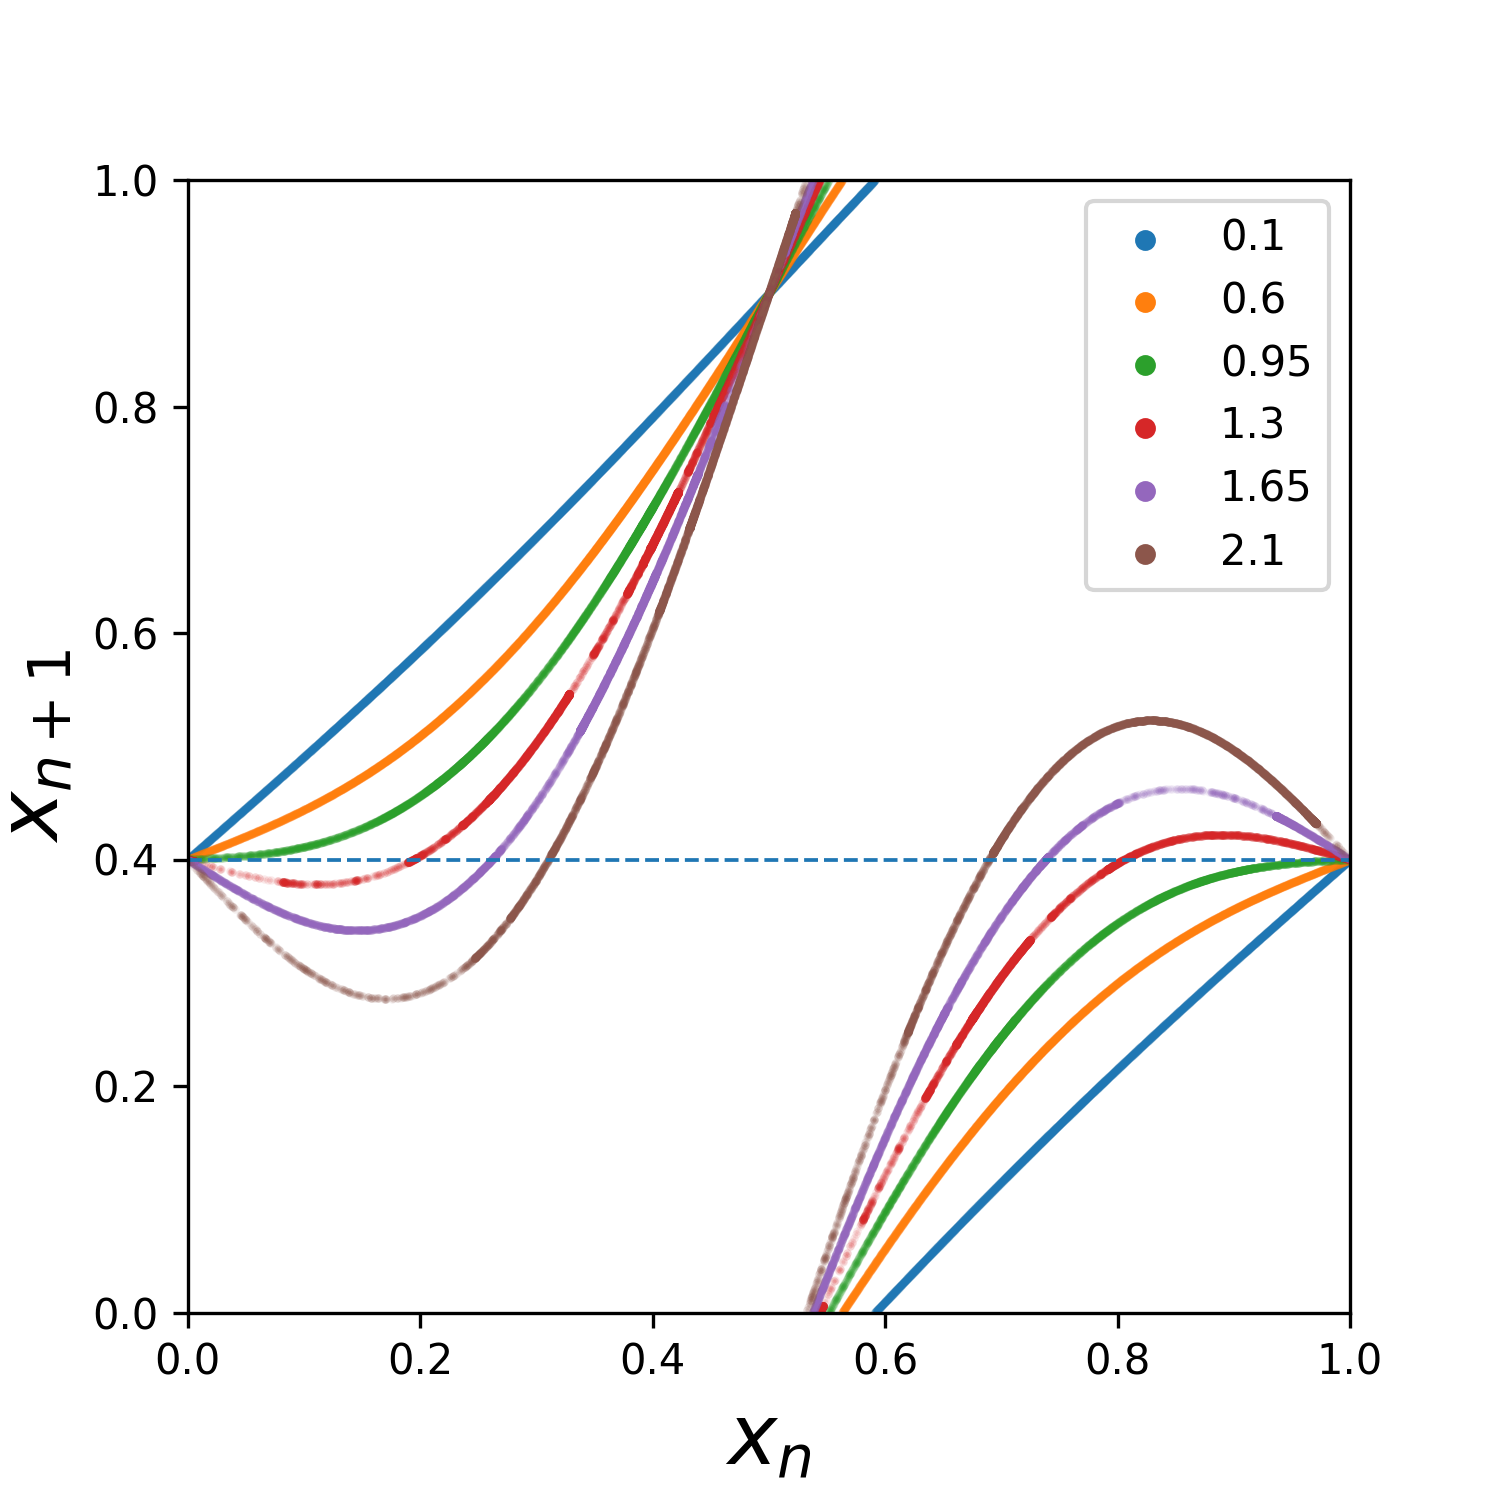
\includegraphics[width=0.3\textwidth]{../figures/chap1/4_3_py.png}
	   \caption{\scriptsize Mappa di Arnold al variare di $k$ con $\omega  = 0.4$ fissato.}
           \label{fig:4_3_py-png}
       \end{figure}
       \noindent
       Come possiamo vedere in figura \ref{fig:4_3_py-png} la mappa non è invertibile per tutti i valori di $k$. \\
       Prendiamo ad esempio la mappa con $k=0.1$ e valutiamo\
       \footnote{Questa corrisponde (circa) alla circle rotation map} il punto $x_n=0$: la linea blu in figura \ref{fig:4_3_py-png}, che rappresenta la mappa, a destra di questo punto vale $\omega+\epsilon$, a sinistra di questo punto vale $\omega-\epsilon$. La pendenza della curva in questo punto è quindi positiva.\\
       La presenza della perturbazione oscillante fa si che i due "rami" della mappa si avvicinino l'un l'altro "distorcendosi", di conseguenza se la perturbazione è abbastanza forte è possibile che in un punto tra $0$ e $1$ il ramo in alto e quello in basso abbiano la stessa $x_{n+1}$: si perde l'iniettività e quindi l'invertibilità.\\
       Nel grafico la perdita di iniettività si ha quando la mappa oltrepassa la linea tratteggiata (che rappresenta la separatrice tra i rami).\\
       Per capire quando questo succede possiamo studiare la pendenza della mappa nei pressi di $x_n = 0$ (considerandola di fatto come una funzione continua).
       \[
	   x_{n+1} = x_n + \omega + k x_n = (1-k) x_n + \omega
       .\] 
       Se in un intorno (destro) di questo punto la pendenza della curva è negativa allora significa che la mappa è scesa sotto $\omega$ e quindi ha perso l'iniettività: deve essere $k\le 1$ per avere pendenza positiva.


